\documentclass[a4paper]{article}

\usepackage[french]{babel}
\usepackage[T1]{fontenc}
\usepackage[utf8]{inputenc}
\usepackage{float}
\usepackage{amsmath}
\usepackage{graphicx}
\usepackage{wrapfig}
\usepackage{lscape}
\usepackage{rotating}
\usepackage{epstopdf}
\usepackage{multirow}
\usepackage{lmodern}
\usepackage[left=3cm, right=3cm, bottom=4cm, top=4cm]{geometry}
\usepackage{array}
\usepackage{pdfpages}

\usepackage[gen]{eurosym}
\DeclareUnicodeCharacter{20AC}{\euro{}}

\usepackage{hyperref}
\hypersetup{
    colorlinks,
    citecolor=black,
    filecolor=black,
    linkcolor=black,
    urlcolor=black
}

\title{Document de planification initiale}

\author
{
    François {\sc Boschet}\\
    Arnaud {\sc Lods}\\
    Marlène {\sc Tuekam}\\
    Alexandre {\sc Bouchet}\\
    Guillaume {\sc Perrudin}\\
    Nguyen {\sc Song Hai}\\
    Romain {\sc Colombat}
}

\date{\today}

\newcommand{\pagevierge}[0]{\newpage\thispagestyle{empty}\null\newpage}

\begin{document}
    % Ouh c'est sale.
    \hypersetup{pageanchor=false}
    
\includepdf[pages=1]{figure/couv.pdf}
    \hypersetup{pageanchor=true}

    \newpage
    \thispagestyle{empty}
    \mbox{}

    \newpage
    % A decommenter pour la release
    \setcounter{tocdepth}{2}
    \tableofcontents
    \setlength{\parskip}{10pt}

    \newpage
    \thispagestyle{empty}
    \mbox{}

    \newpage
    \section{Introduction}

	\section{Rappel de la phase d'analyse}
\label{sec:rappel}
	
    \section{Recherche de documents}
\label{sec:recherche}

La plateforme joue en quelque sorte le rôle d'un moteur de recherche. L'idée est de fournir aux utilisateurs une recherche riche et diverse qui lui permettra de trouver efficacement des journaux, des articles ou des revues de presse qu'il souhaiterait consulter. On veut donc permettre à l'utilisateur d'effectuer trois types de recherches; suivant le type des documents qu'il recherche. Cette fonctionnalité est une fonctionnalité importante pour l'utilisateur, l'enjeu étant de lui permettre de trouver le plus efficacement possible des documents qui peuvent l'intéresser.

Nous avons décidé qu'un utilisateur ne pourra pas chercher en même temps des 'articles' et des 'journaux' pour distinguer ces différents types et d'éviter de rendre trop de résultats inintéressants. Suivant le type de document recherché l'utilisateur disposera de plusieurs filtres qui seront mis à jour sur la page ; ces filtres dépendront bien évidemment du type de document sélectionné.

Il sera bien évidemment possible de trier les résultats par date ; par ordre chronologique de parution ou non.

\subsection{Recherche de journaux}
\label{sec:recherche_journal}

La première recherche élémentaire est celle des journaux. L'utilisateur, en arrivant sur cette page, devra être capable de pouvoir chercher l'édition d'un journal qui l'intéresse. Pour ça, il pourra effectuer une recherche sur le nom de celui-ci, mais aussi sur la date. Si le nombre de journaux différents n'est pas trop important, l'utilisateur disposera directement d'une liste de tous les journaux. Pour la date, il aura le choix de la filtrer suivant trois catégories : 'AVANT', lui permettant de trouver toutes les éditions sorties avant une certaine date, 'APRES', permettant au contraire d'obtenir les éditions sorties après la date écrite. Enfin 'ENTRE' permettra de chercher des journaux édités entre deux dates précises. Pour rechercher sur une date, l'utilisateur devra au minimum rentrer l'année et pourra jusqu'à rentrer le jour et le mois. Il sera bien évidemment possible de chercher plusieurs journaux. Un utilisateur pourra chercher des éditions de 1940 de 'Libération' et du 'Canard enchaîné' en même temps ; il suffira de sélectionner ces deux-là dans la liste de journaux avant de lancer la recherche.

Les résultats affichés donneront le nom du journal et sa date de parution. Cliquer sur un des résultats permettra d'arriver sur la page de consultation de document pour lire ce dernier.

En résumé, la recherche de journaux s'effectuera sur deux attributs :
\begin{itemize}
	\item Le nom du journal
	\item La date d'édition
\end{itemize}

\subsection{Recherche d'articles}
\label{sec:recherche_article}

La seconde recherche essentielle de la plateforme sera la recherche d'articles. Habituellement un utilisateur lisant un journal se retrouvera assez souvent à chercher des informations sur des évènements particuliers qui auraient pu se dérouler. Dans ce but, ou dans le cas où un utilisateur souhaiterait créer une revue de presse d'articles spécifiques, il est nécessaire de permettre à l'utilisateur de pouvoir chercher avec de nombreux filtres différents des articles.

Les deux premiers filtres sont les mêmes que pour les journaux et suivent le même fonctionnement; l'utilisateur pourra chercher des articles d'un (ou de plusieurs) journal spécifique et suivant une date spécifique. Un autre filtre essentiel pour cette recherche est bien évidemment la recherche sur un titre d'article. L'utilisateur aura un champ qui recherchera donc spécifiquement sur le titre des articles stockés. L'utilisateur pourra aussi effectuer une recherche sur le contenu de l'article. À l'instar d'une recherche google, il sera possible de rentrer du texte qui sera cherché dans le texte d'un article; et les occurrences des mots recherchés seront mis en évidence (gras) dans le résultat de recherche. Un autre élément de recherche, plus spécifique, mais qui peut rester utile (dans le cadre d'une revue de presse sur une personne), est la recherche sur l'auteur d'un article. Un champ sera disponible pour chercher des articles écrits par une certaine personne. Enfin, il sera possible pour l'utilisateur de chercher des articles suivant les tags qui lui ont été associés. À la manière de twitter, une auto-complétion lui permettra de rentrer des tags qui ont été définis auparavant, cela lui permettra d'être sûr de ne pas rentrer des tags qui n'existeraient pas.

Les résultats affichés contiendront le nom de l'article, le nom du journal d'appartenance, la date de parution, l'auteur, la liste des tags associés à celui-ci et quelques lignes de début de l'article. Si une recherche dans le contenu de l'article était effectuée, alors à la place les lignes affichées présenterons le contexte dans lequel les mots ont été trouvés. Cliquer sur un résultat amènera l'utilisateur sur la visionneuse de document avec l'article pré-sélectionné.

Il sera par ailleurs possible de trier ces articles en deux catégories; les articles appartenant à une revue de presse et les autres. Les résultats d'articles appartenant à une revue de presse auront un fond coloré, permettant de les identifier.

En résumé, la recherche d'articles s'effectuera sur six attributs :
\begin{itemize}
	\item le journal dans lequel il est paru;
	\item la date de parution;
	\item le titre de l'article;
	\item les tags associés à l'article;
	\item le contenu de l'article;
	\item l'auteur de l'article.
\end{itemize}

\subsection{Recherche de revues de presse}
\label{sec:recherche_revue}

Le dernier type de recherche disponible pour l'utilisateur se trouve être la recherche sur les revues de presse. Cela lui permettra de ne pas avoir à chercher dans la liste des revues de presse une revue qui l'intéresse. Cette recherche est assez simple; l'utilisateur pourra effectuer une recherche sur le nom de la revue de presse et sur la description de celle-ci.

Les résultats affichés contiendront le nom de la revue de presse, sa description et les trois premiers articles de celle-ci. Cliquer sur un résultat amènera l'utilisateur sur la page de la revue de presse. Il sera par ailleurs possible de trier les résultats obtenus suivant la date de création de la revue de presse, mais aussi la date de la dernière modification de celle-ci.

En résumé, la recherche de revues de presse s'effectuera sur deux attributs :
\begin{itemize}
	\item Le nom de la revue de presse
	\item La description de la revue de presse
\end{itemize}
\bigskip
\par
D'après les spécifications pour la fonctionnalité de recherche; on arrive à un croquis de la page rassemblant toutes ces fonctionnalités qui devrait prendre la forme suivante. (Figure \ref{fig:recherche_img})

    \begin{figure}[H]
        \centering
        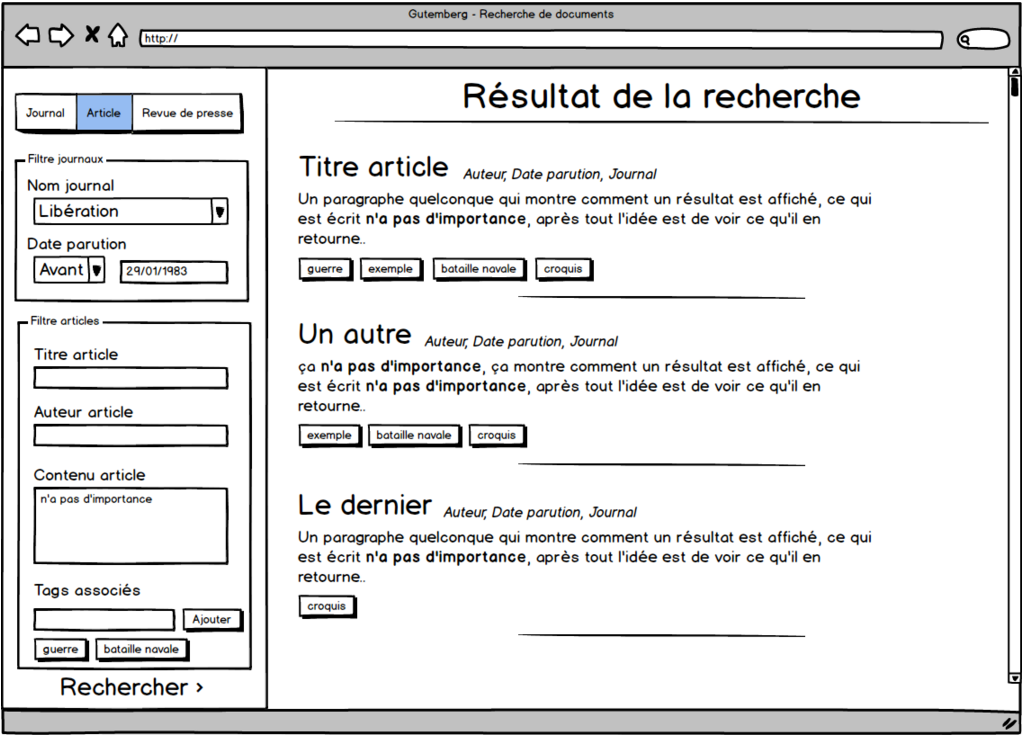
\includegraphics[width=\textwidth]{figures/recherche.png}
            \caption{Page de recherche d'un article}
            \label{fig:recherche_img}
    \end{figure}

    \section{Consultation de documents}
\label{sec:consultation}

La page de consultation de documents est une page générique devant proposer trois modes de consultation :
\begin{itemize}
\item Article
\item Journal
\item Revue de presse
\end{itemize}

Il est important d’apporter une valeur ajoutée à cette consultation de document. Trois objectifs ont donc été définis :
\begin{itemize}
\item Informer l’utilisateur sur le document qu’il consulte
\item Consulter le document
\item Guider l’utilisateur en lui proposant de consulter d’autres documents
\end{itemize}
C’est selon ces trois objectifs que l’interface et les fonctionnalités ont été imaginées.


\subsection{Informer}
\label{sec:consultation_informer}
	La consultation d’un document ne doit pas se cantonner à un simple affichage d’image. Il est également important d’informer l’utilisateur sur ce qu’il consulte. La partie gauche de la page y sera dédiée. Celle-ci sera rétractable afin de laisser à la visionneuse d'image plus de place sur la page quand l'utilisateur n'a pas besoin de ces informations.
On y trouvera des informations concernant :
\begin{itemize}
\item Le journal en cours de consultation : titre, date.
\item La page de journal en cours de consultation : liste des articles et de leurs éventuelles images sous forme d'arborescence. L'utilisateur pourra cliquer sur un de ces articles pour y accéder : la visionneuse de la page zoomera alors sur cet article.
\item L’article en cours de consultation : titre, tags.
\end{itemize}
\bigskip
\par
	Cette liste d’information n’est pas exhaustive, elle dépendra des méta données qui nous serons mises à disposition.
	L’utilisateur pourra également être acteur de la classification des articles. En effet, l'utilisateur pourra aussi ajouter des tags et également en supprimer. En effet, lorsque celui-ci sélectionne un article, il aura alors la possibilité d'y ajouter des tags. À la manière de Twitter, la saisie de tags sera facilitée grâce à l'auto-complétion afin de ne pas avoir plusieurs tags similaires ayant différentes orthographes dans la base de données. Il lui sera aussi possible d’ajouter l’article à une revue de presse ou à ses favoris. Il pourra alors choisir une revue de presse en effectuant une recherche ; les revues de presse qu’il a créées ou celles auxquelles il a participé seront proposées en premier dans les résultats de recherche. S’il ne trouve pas la revue de presse qui lui convient, l’utilisateur aura la possibilité d’en créer une (voir maquette en bas à gauche). 

	En cliquant sur un article dans la liste des articles de la page, ce dernier sera mis en évidence par un calque transparent. Si des calques étaient déjà appliqués, ceux-ci seront supprimés pour ne laisser que l'article concerné et le repérer plus facilement.

\subsection{Consulter}
\label{sec:consultation_consulter}
La fonctionnalité principale est bien sûr de consulter des documents. Le milieu de la page y sera consacré.
L’interface de visualisation affichera une page de journal avec un focus différent selon le mode de lecture :
\begin{itemize}
\item “Article” et “Revue de presse” : la visionneuse zoome sur l’article concerné. Celui-ci sera mis en évidence par un calque transparent coloré.
\item “Journal” : la visionneuse affiche la première page du journal, sans zoom.
\end{itemize}
\bigskip
\par
Si l’utilisateur survole un autre article, celui-ci sera également mis en évidence par un calque.
	L’utilisateur aura aussi la possibilité de zoomer/dézoomer et de se déplacer dans la page, ainsi que d’effectuer une recherche textuelle dans la page. Pour avoir une utilisation plus fluide, l'utilisateur pourra double-cliquer sur un article, et ce afin de zoomer directement sur ce dernier. Double-cliquer à nouveau dessus réinitialisera le zoom afin d'avoir à nouveau la page d'ensemble. Si la lecture est en mode “Revue de presse”, il sera possible de passer à l’article précédent ou suivant de la revue de presse. Dans tous les cas, l'utilisateur pourra naviguer entre toutes les pages du journal. Par défaut, en arrivant sur une page, tous les articles seront mis en évidence avec des calques transparents de couleurs différentes.

\subsection{Guider}
\label{sec:consultation_guider}

	Tous les utilisateurs ne viendront pas en sachant quel article ils souhaitent consulter ; beaucoup d’entre eux voudront simplement découvrir. Dans cette mesure, il semble important de guider l’utilisateur. La partie droite de la page y sera consacrée. Par ailleurs, cet espace permettra aussi à l'utilisateur de découvrir l'architecture de la page qu'il est en train de lire ; il pourra ainsi voir la liste des articles contenus dans la page. En cliquant sur un article, celui-ci sera mis en évidence sur la page grâce à un calque transparent coloré.

	Trois fonctionnalités participeront à ce guidage :
\begin{itemize}
\item Articles similaires : une sélection d’articles similaires à celui en cours de lecture sera proposée à l’utilisateur. Ces recommandations pourront s’effectuer selon plusieurs critères : ressemblances de mots, journaux, périodes ou tags identiques.
\item Revues de presses associées : une liste des revues de presse contenant l’article en cours de visualisation sera proposée à l’utilisateur. L’idée est de le diriger vers des thématiques pouvant potentiellement l’intéresser.
\item Articles de la revue de presse : si la lecture est en mode “Revue de presse”, l’utilisateur aura accès à la liste des articles de celle-ci.
\end{itemize}

\bigskip

    \begin{figure}[H]
        \centering
        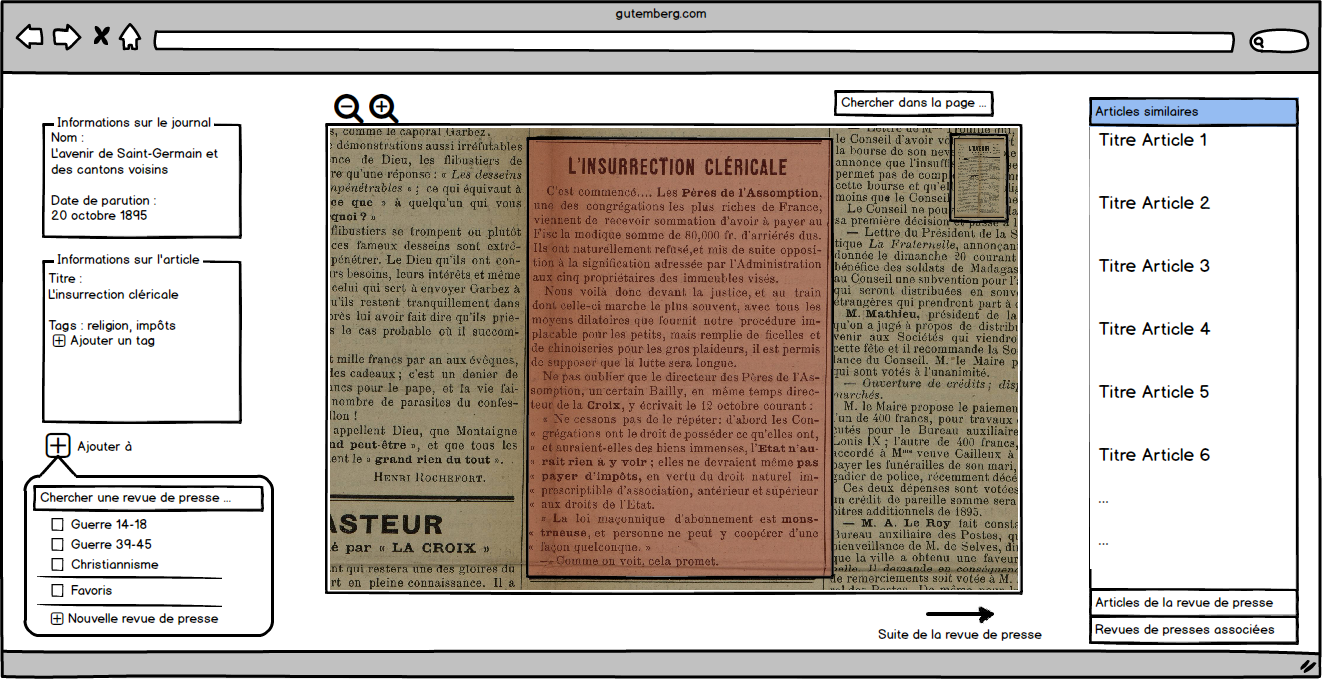
\includegraphics[width=\textwidth]{figures/consultation.png}
            \caption{Page de consultation de documents}
            \label{fig:consultation}
    \end{figure}

    \section{Les revues de presse}
\label{sec:revue}

La principale fonctionnalité innovante de notre plateforme de consultation de journaux anciens est la possibilité de
créer et de partager des revues de presse.

Une revue de presse est, basiquement, une liste d'articles de journaux regroupés ensemble par un ou plusieurs utilisateurs autour d'une thématique précise,
comme par exemple une date, un événement ou une zone géographique.

La création des revues de presse pourra se faire à deux moments distincts. En cliquant sur un bouton depuis le menu principal, l'utilisateur se verra redirigé vers une page de création de revue de presse. Cette page contiendra des champs pour nommer la revue de presse et lui mettre un commentaire descriptif. L'utilisateur pourra ensuite ajouter des articles à sa revue de presse et pourra la consulter depuis son profil ou depuis le moteur de recherche. La deuxième manière d'accéder à la page de création d'une revue de presse sera à partir de la page de visualisation, lors du clique sur le bouton d'ajout d'un document à une revue de presse. Il s'agit de la même page que décrite précédemment,
la seule différence étant que la revue de presse sera initialisée avec le-dit document.

Il y aura plusieurs moyens d'ajouter un document à une revue de presse :  

\begin{itemize}
  \item cliquer sur le bouton d'ajout présent sur la page de visualisation et choisir la
revue de presse à laquelle contribuer.
  \item cliquer sur le bouton d'ajout directement présent depuis le moteur de recherche et choisir
à quelle revue de presse contribuer.
  \item cliquer depuis la page récapitulative d'une revue de presse sur les boutons d'ajout de chaque document.
\end{itemize}
Depuis la page récapitulative d'une revue de presse, il sera aussi possible, pour le créateur de la revue de presse, de retirer un article de
la revue de presse.

La page de visualisation d'une revue de presse serae composé du titre, de la description de la revue de presse et d'une liste comprenant les articles
de cette revue de presse. Depuis cette page il sera possible de modifier le titre, la description et de retirer un article sur cette revue de presse.

    \begin{figure}[H]
        \centering
        
\includegraphics[width=\textwidth]{figures/manquant.png}
            \caption{Schéma manquant}
            \label{fig:manquant}
    \end{figure}

    \section{Itération 4 : page d'accueil}

    \section{Itération 5 : gestion d'utilisateur}

    \section{Planification du projet}
\label{sec:orga}

	Les différents délivrables du projet 4INFO imposent une gestion de projet suivant un modèle de cycle en V. Cependant, nous sommes libres d'adapter nos propres méthodes de développement 

	Ici, nous avons de nombreuses fonctionnalités que nous allons être amené à réaliser. Il est donc nécessaire de penser à une bonne méthode de gestion lors du développement. Cela nous permettra de gérer au mieux le temps qui nous est imparti en prenant en compte les ressources que nous avons à disposition notamment humaines. D'un côté, il est nécessaire d'évaluer l'importance de chaque fonctionnalité, définie bien précisément, et de l'autre, la partie la plus complexe, il nous faut estimer la durée pour réaliser chaque tâche.

	En respectant un modèle de cycle en V, nous nous retrouverions donc à développer la plateforme, puis à effectuer différentes séries de tests avant de la délivrer. Le problème de cette méthode est que nous allons devoir faire une sélection de fonctionnalités à développer, s'y tenir, et un livrable ne sera fournit qu'à la fin. Entre autre, nous ne pourrons avoir un retour sur l'application que lorsque le développement sera fini. Il sera impossible d'inférer sur les fonctionnalités puisqu'il n'y aura aucun retour durant le temps de développement. 

	C'est pourquoi nous pensons planifier le développement de l'application en se basant sur les méthodes agiles. Nous aurons donc une liste de fonctionnalités, triée suivant leur importance et leur difficulté à être développées. En considérant les ressources mises à disposition, nous délivrerons et effectuerons en continue des tests pour chacune des fonctionnalités. Ainsi il sera possible de présenter l'avancement au milieu du projet à nos encadrants, et il serait possible de redéfinir certaines priorités pour les fonctionnalités restantes, ou en rajouter par la suite si nous prenons de l'avance sur le développement. Si celles-ci se trouvent être plus intéressantes (ou plus faciles), nous pourrions nous retrouver à les développer en priorité par rapport à des fonctionnalités définies avant. Enfin, cela permet à un instant T d'avoir un produit fonctionnel.

	En faisant une liste non exhaustive de tâches globales (on ne détaille pas encore toutes les sous-tâches de développement qu'une tâche implique, et les tests sont inclus dans le temps de la tâche), et en les ordonnant de manière à obtenir une plateforme qui contiendra au fur et à mesure de plus en plus de fonctionnalités en partant des plus importantes; on arrive à ce schéma de planification.

	\begin{figure}[H]
        \centering
        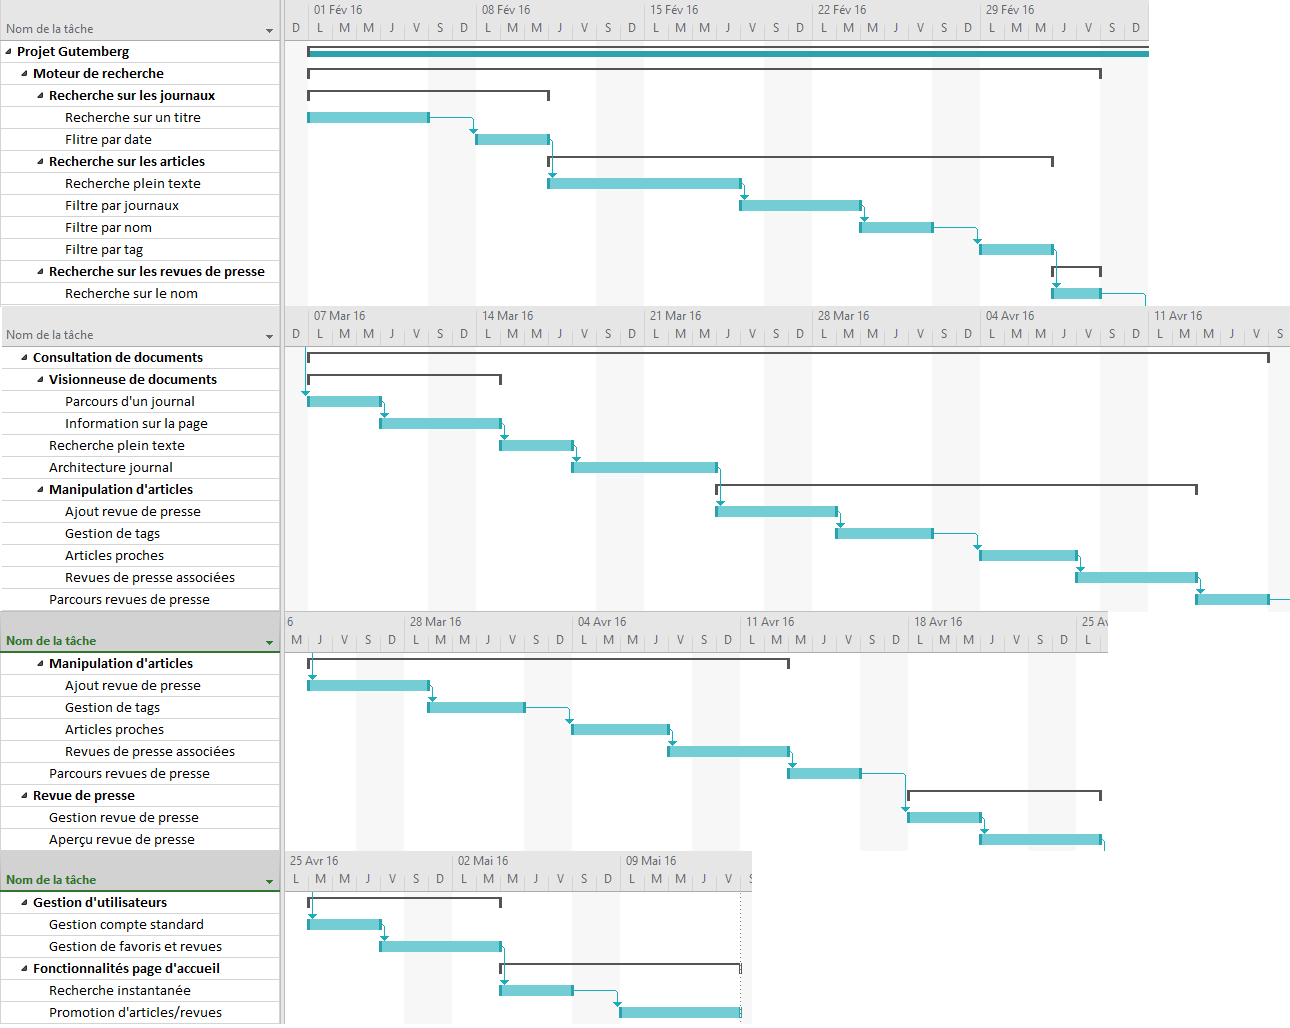
\includegraphics[width=1.3\textwidth, angle=90]{figures/plan.png}
            \caption{Plannification}
            \label{fig:plan_recherche}
    \end{figure}

	\section{Conclusion}
\label{sec:conclusion}
	
	Ce rapport et les deux présentations qui donnent suite à ce dernier représentent la fin de la phase d'analyse et de spécifications. Nous avons vu et estimé la durée de chacune des tâches pour chaque itération du projet. Cela nous a permis d'établir une planification initiale des tâches pour le reste du projet, du début de la phase de conception jusqu'au rendu de la dernière version du projet.

	L'étape suivante du projet sera donc la phase de conception de celui-ci. Nous établirons l'architecture de la base de données que nous utiliserons, nous définirons les différents modules de l'application, et la façon dont ceux-ci communiquent entre eux, et nous procéderons à l'installation de l'environnement de travail pour la suite du projet.
    % Manoucherie incoming
    \pagevierge
    \ifthenelse{\isodd{\thepage}}
    {\pagevierge}
    {}
    
\includepdf[pages=2]{figure/couv.pdf}
\end{document}
